
The HotPy virtual machine is high-performance optimising VM for Python. In order that optimisations that it performs can be analysed and trusted to be correct, there must be some way to describe the state of the VM.

\subsection{The High Level Model}

The HotPy VM consists of a single, global garbage-collected heap of objects and one or more GVMT-level threads of execution and one or more 
HotPy threads. Each GVMT-level thread executes one HotPy thread at a time. 

In the HotPy VM model, each GVMT-level thread consists of a single reference to HotPy \verb|thread| object and the GVMT-provided data-stack.
The GVMT executes bytecode using a GVMT-generated interpreter, or as machine code generated by a compiler generated by the GVMT compiler-generator.
The currently executing bytecode is managed by the GVMT-generated components, but the bytecode-instruction pointer can be read at any point by the HotPy VM.

Each \verb|thread| object corresponds one-to-one with a HotPy thread.
Machine-level threads do not map one-to-one to Python threads. Allocation of objects and garbage-collection is managed by the GVMT upon which HotPy is built.

\subsection{Objects}

Although the HotPy VM, can support an infinite number of classes,
the following classes are required to describe the execution model of the HotPy VM.
All objects are heap allocated and fully managed by the GVMT.

\begin{myitemize}
\item object
\item type
\item thread
\item frame
\item function
\item code\_object
\item exception\_handler
\end{myitemize}

The following classes are required  to describe the optimisation passes.
\begin{myitemize}
\item dict
\item dict\_values
\item dict\_keys
\item int
\item float
\end{myitemize}

\subsubsection{The object class}
The \verb|object| class is the root of the inheritance hierarchy in Python. All HotPy objects include the single \verb|class| field. 
Many objects also have a \verb|dict| field which refers to the instance dictionary for that object.
Whether or not an object has a \verb|dict| field is recorded in its \verb|class|.

\subsubsection{The type class}
Since Python is a dynamic language, classes are objects like all other objects. All classes have \verb|type| as their \verb|class|. \verb|type| is its own class. The \verb|type| class has various fields that are required for describing objects to the garbage collector and other book-keeping details. The following fields are relevant to the HotPy VM model.
\begin{description}
\item[dict\_offset] Records the offset of the \verb|dict| field in instances of this class, or zero if instances do not have dictionaries.
\item[dict] The \verb|dict| field of a \verb|type| object is special.
It describes the attributes of all instances of the class (\verb|type| object), rather than the class itself.
\item[mro] Abbreviation for method resolution order. An array of \verb|type| objects, used when resolving attributes. \verb|mro| contains a linearisation of the super-classes of the type (including itself);  \verb|t.mro[0]| is \verb|t| and \verb|t.mro[n-1]| is the \verb|object| class.
To lookup the class attribute \verb|cls.x| look for 'x' in \verb|cls.mro[0].dict|, then\verb|cls.mro[1].dict|, through to \verb|cls.mro[n-1].dict|.
\end{description}

\subsubsection{The thread class}
Each thread object contains a number fields which are necessary for thread switching, debugging and optimization.
In order to describe the VM, only one is necessary, \verb|current_frame| which refers to the \verb|frame| for the currently executing function.
Most of the state of a HotPy thread is stored in the stack of \verb|frame|s, implemented as a singly linked list. Each \verb|thread| object has a \verb|current_frame| field which refers to the currently executing frame.

\subsubsection{The frame class}

The following fields of the \verb|frame| class are relevant to the HotPy execution model.
\begin{description}
\item[length] The number of local variables.
\item[locals\_array] The local variable array
\item[next\_ip] A pointer to the next instruction (bytecode) to be executed.
\item[exception\_handlers]  A singly linked list of exception handlers (may be empty).
\item[code] Holds references to built-in and module scopes.
It also contains a \verb|dict| for the local variables, for those frames that cannot store their locals in the locals\_array.
\item[back] A reference to the caller frame.
\item[depth] The depth of the frame. depth = back$\rightarrow$depth + 1
\end{description}

\subsubsection{The function class}

The \verb|function| class describes a Python function. Most of the details of the Python function are contained in the \verb|code_object| object which includes the actual bytecodes, as well as the number of parameters and number of local variables. The \verb|function| contains those details that cannot be determined statically from the source code, such as default values.
The \verb|function| class has the following fields that are relevant to the HotPy VM model.
\begin{description}
\item[code] The code object for this function
\item[defaults] Default values for unspecified parameters
\item[scopes] The built-in and module-level dictionaries for this function.
\item[closure] If this is a nested function, this refers to the frame in which this function object was created.
\end{description}

\subsubsection{The code\_object class}

The \verb|code_object| class describes the static parts of a Python function. The  \verb|code_object| class has the following fields:
\begin{description}
\item[kind] A code describing the parameter passing conventions for this function. There are four possibilities: surplus positional arguments may raise an exception or be passed in a tuple; surplus named arguments may raise an exception or be passed in a dictionary.
\item[param\_count] The number of parameters declared for this function.
\item[locals\_count] the number of local variables declared in this function
\item[bytecodes] The bytecode instructions for this code\_object.
\end{description}

\subsubsection{The exception\_handler class}
The \verb|exception_handler| class is unique in the HotPy VM model in that is not a class in the standard Python library, it is purely internal to the HotPy VM.

The \verb|exception_handler| class has the following fields:
\begin{description}
\item[data\_stack\_depth] The number of values on the data stack
\item[ip] The first bytecode to be executed if an exception is raised.
\item[next] The next \verb|exception_handler| object in the linked list.
\end{description}

\subsection{Execution}

\subsubsection{Threads}

Each HotPy thread is described by a single \verb|thread| object. The current state of execution is described by a stack, implemented as singly linked list, of \verb|frame| objects.

Before describing an executing thread, it is easier to describe a suspended thread. For each \verb|frame| in the stack, the \verb|next_ip| field of each frame points to the next bytecode to be executed when that frame is the current frame. For each \verb|try| statement that has been executed and is still in scope, there exists one \verb|exception_handler| object, each of which is attached to the relevant frame. See Figure \ref{fig:stack}

When a thread is executing, the \verb|next_ip| field of the current frame is ignored,
instead the GVMT handles the instruction pointer, \verb|current_ip|.
A thread is resumed by setting the \verb|current_ip| to the \verb|next_ip| of the current frame, then executing as normal.
A thread is suspended by setting the \verb|next_ip| of the current frame to the \verb|current_ip|.
Threads cannot be suspended in mid-bytecode.

\begin{figure}[htb]
 \centering
 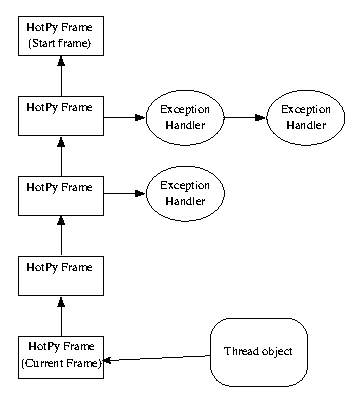
\includegraphics[scale = 1.1]{./vm_stack.eps}
 \caption{A HotPy Thread\label{fig:stack}}
\end{figure}

\subsubsection{Starting a Thread}
Execution of thread is started by calling the \verb|py_call|. This sets up the current thread, pushing a new \verb|frame| onto the frame stack, initialising it and calling the \verb|super_interpreter| function to commence execution.

\subsubsection{Bytecodes}

Execution of a HotPy thread occurs by the successive execution of individual bytecodes. Each bytecode transforms the state of the VM. 

Bytecodes are described either in terms of the arithmetic or bitwise operations they perform on the objects or by the transformations they make to the VM state. Many bytecodes have complex semantics, they perform operations by performing a sequence of transformations 

Many bytecodes have simple semantics, such as reversing the top two elements of the stack. The remainder are either specialised opcodes used by the optimisers, or bytecodes that change the state of the VM; these are covered in more detail. A complete description of all instructions in included in Appendix \ref{app:instructions}.

\subsubsection{Calling Functions}
The \verb|call| instruction expect three values to be on the stack, the object to called, a tuple of positional parameters and a dictionary of named parameters. The object is third on stack, the dictionary top of stack. 
The \verb|call| instruction has varying semantics depending on the object being called.

If a callable is a Python function, then a new \verb|frame| is created, taking its size from the code\_object of the function. The parameters are then filled in from the tuple, dictionary and any defautls defined in the function. The state of the VM is then changed as follows.
The \verb|next_ip| field of the current frame is set to the address of the instruction following the \verb|call| instruction. The \verb|back| field of the new frame is set to the current frame. The current frame is set to the new frame. Execution then proceeds from the first instruction in the code\_object of the called function. Figure \ref{fig:py-call} shows the change in state.

\begin{figure}[htb]
  \begin{center}
    \subfigure[Before call]{\centering\label{fig:fib-before}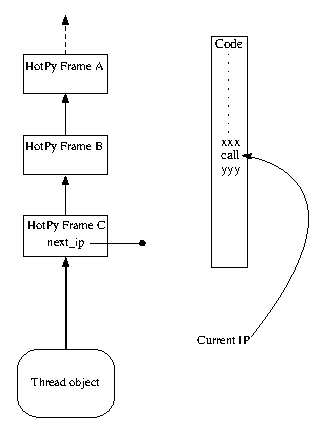
\includegraphics[scale=1.2]{./before.eps}}
    {\hspace{0.1cm}}
    \subfigure[After call]{\centering\label{fig:fib-after}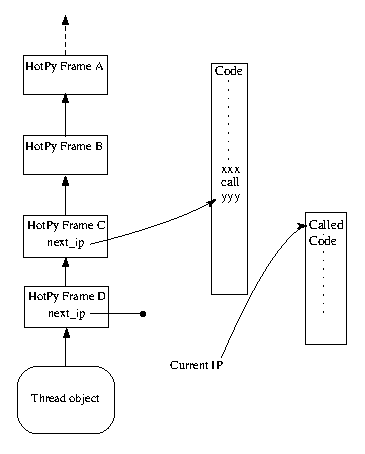
\includegraphics[scale=1.2]{./after.eps}}
  \end{center}
  \caption{Call sequence}
  \label{fig:py-call}
\end{figure}

\subsubsection{Calling native (C) code}
In order to implement Python properly, particularly to support library code written in C, it must be possible to call C ocde from Python and vice versa. Calls to C ocde are effectivel opaque to the VM. When calling a C function, the parameters are popped from the stack and passed to the function (this is handled by the GVMT).

C code may need to call back into Python code. For example, the \verb|dict.__getitem__| method is implemented in C for speed, but may need to call the \verb|__hash__| method of a class implemented in Python.

C code calls back into the VM, by calling a Python function using the \verb|py_call| function. This creates a new HotPy frame, which is pushed to the frame stack, and calls the \verb|super_interpreter| function to resume execution.


